% main.tex
% Fichero principal de transparencias (incluye a todos los dem�s).

% Compilar a .pdf con LaTeX (pdflatex)
% Es necesario instalar Beamer (paquete latex-beamer en Debian)
%

% Gr�ficos:
% Los gr�ficos pueden suministrarse en PNG, JPG, TIF, PDF, MPS
% Los EPS deben convertirse a PDF (usar epstopdf)
%
\documentclass{beamer}
\usetheme{Warsaw}
\beamertemplatenavigationsymbolsempty
\setbeamertemplate{headline}{}
\useoutertheme{infolines}
%\usebackgroundtemplate{\includegraphics[width=\paperwidth]{format/libresoft-bg-soft.png}}
\usepackage[spanish]{babel}
\usepackage[latin1]{inputenc}
\usepackage{graphics}
\usepackage{amssymb} % Simbolos matematicos

\newcommand{\asignatura}{Pr�cticas educativas abiertas}
\newcommand{\grado}{Itinerario formativo en innovaci�n did�ctica (URJC)}

%\definecolor{libresoftgreen}{RGB}{162,190,43}
%\definecolor{libresoftblue}{RGB}{0,98,143}

%\setbeamercolor{titlelike}{bg=libresoftgreen}

%% Metadatos del PDF.
\hypersetup{
  pdftitle={\asignatura},
  pdfauthor={Jes�s M. Gonz�lez Barahona, Gregorio Robles},
  pdfcreator={GSyC, Universidad Rey Juan Carlos},
  pdfproducer=PDFLaTeX,
  pdfsubject={\asignatura},
}
%%


%%%%%%%%%%%%%%%%%%%%%%%%%%%%%%%%%%%%%%%%%%%%%%%%%%%%%%%%%%%%%%%%
%%%%%%%%%%%%%%%%%%%%%%%%%%%%%%%%%%%%%%%%%%%%%%%%%%%%%%%%%%%%%%%%
% include-only                                                 %
%%%%%%%%%%%%%%%%%%%%%%%%%%%%%%%%%%%%%%%%%%%%%%%%%%%%%%%%%%%%%%%%
%%%%%%%%%%%%%%%%%%%%%%%%%%%%%%%%%%%%%%%%%%%%%%%%%%%%%%%%%%%%%%%%
%\includeonly{intro}

\AtBeginSection[]
{
\begin{frame}<beamer>
\begin{center}
{\Huge \insertsection}
\end{center}
\end{frame}
}


\begin{document}

\title[\asignatura]{\asignatura}
\subtitle{\grado}
\author[GSyC]{Jes�s M. Gonz�lez Barahona, Gregorio Robles Mart�nez}
\institute{GSyC, Universidad Rey Juan Carlos}

\date{Junio 2015}


\frame{
\maketitle

\begin{center}

\includegraphics[width=6cm]{format/gsyc-urjc}
\end{center}
}


% Si el titulo o el autor se quieren acortar para los pies de p�gina
% se pueden redefinir aqu�:
%\title{Titulo corto}
%\author{Autores abreviado}


%% LICENCIA DE REDISTRIBUCION DE LAS TRANSPAS
\frame{
~
\vspace{3cm}

\begin{flushright}


\includegraphics[width=2.2cm]{format/by-sa}
 \\

\begin{footnotesize}
\copyright 2014-2015 Jes�s M. Gonz�lez Barahona y Gregorio Robles. \\

Algunos derechos reservados. Este art�culo se distribuye bajo
la licencia ``Reconocimiento-CompartirIgual 3.0 Espa�a'' de Creative Commons,
disponible en \\
{\small \url{http://creativecommons.org/licenses/by-sa/3.0/es/deed.es}}

Este documento (o uno muy similar) est� disponible en \\
\url{http://LibreLearning.github.io}

\end{footnotesize}
\end{flushright}

}
%%

\frame{
\tableofcontents
}

%%%%%%%%%%%%%%%%%%%%%%%%%%%%%%%%%%%%%%%%%%%%%%%%%%%%%%%%%%%%%%%%
%%%%%%%%%%%%%%%%%%%%%%%%%%%%%%%%%%%%%%%%%%%%%%%%%%%%%%%%%%%%%%%%
% lista de temas                                               %
%%%%%%%%%%%%%%%%%%%%%%%%%%%%%%%%%%%%%%%%%%%%%%%%%%%%%%%%%%%%%%%%
%%%%%%%%%%%%%%%%%%%%%%%%%%%%%%%%%%%%%%%%%%%%%%%%%%%%%%%%%%%%%%%%
% $Id$
%


\usebackgroundtemplate{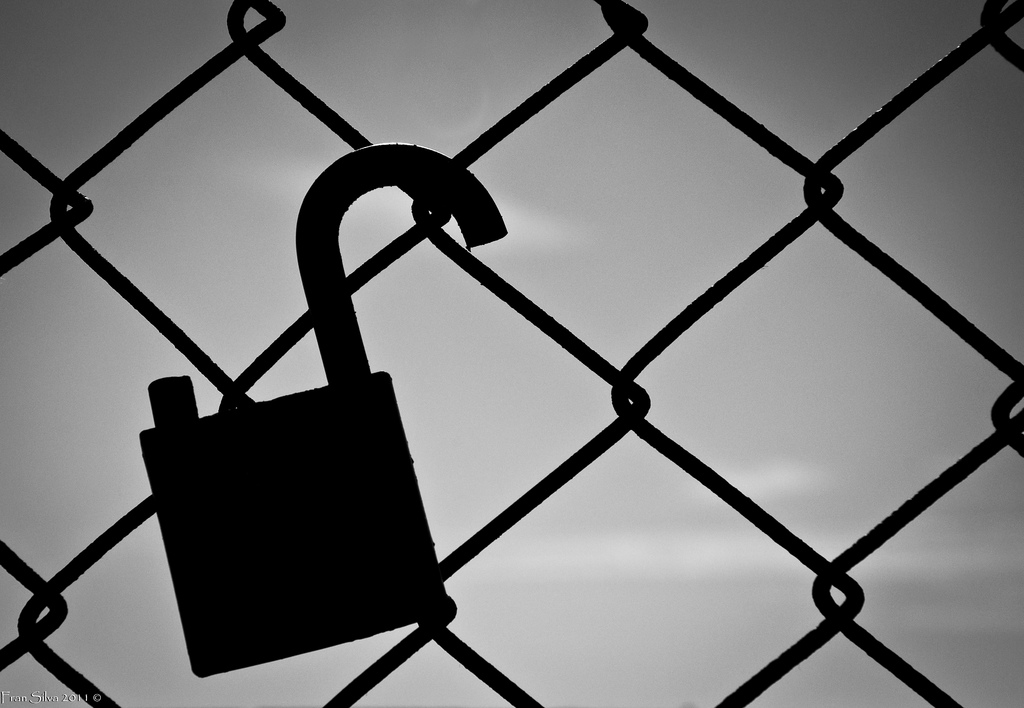
\includegraphics[width=13cm]{figs/candado}}
{\bf
  \textcolor[rgb]{1,1,1}{
    \section{Presentaci�n}
  }
}

\usebackgroundtemplate{}

%%---------------------------------------------------------------

\begin{frame}
\frametitle{Pr�cticas abiertas}

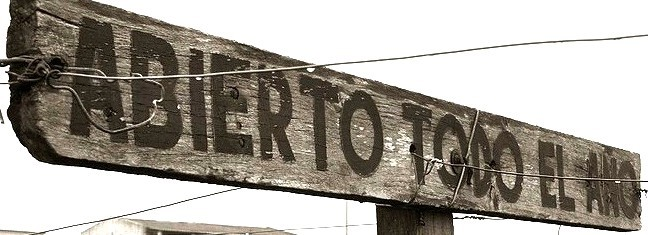
\includegraphics[width=6.5cm]{figs/abierto-todo}

{\Large
\begin{itemize}
\item Abiertas hacia los alumnos:
  \begin{flushright}
    nuevos roles, m�s activos \\
    aprovechar las habilidades del alumno \\
  \end{flushright}

    
\item Abiertas hacia los dem�s:
  \begin{flushright}
    trascender las paredes del aula
    aprovechar Internet
  \end{flushright}
\end{itemize}
}
\end{frame}

%%---------------------------------------------------------------

\begin{frame}
\frametitle{Trasladando desde el software libre}


\begin{itemize}
\item Abiertas hacia los alumnos:
  \begin{flushright}
    aprendizaje con ayuda de tus pares \\
    difuminaci�n de papeles (profesor / alumno) \\
  \end{flushright}
\item Abiertas hacia los dem�s:
  \begin{flushright}
    escrutinio p�blico \\
    creaci�n de comunidad \\
  \end{flushright}
\end{itemize}

\end{frame}

%%---------------------------------------------------------------

\begin{frame}
\frametitle{Hacia los alumnos}


Actores principales del aprendizaje

\begin{itemize}
\item Tienen muchas habilidades muy �tiles
\item Saben muy bien qu� les falta \\
  (incluso cuando no lo saben) \\
\item Comprenden muy bien a otros alumnos
\item El profesor atento a \\
  completar, corregir, comentar \\
\end{itemize}

\begin{flushright}
  M�s posibilidades conllevan m�s responsabilidades
\end{flushright}

\end{frame}

%%---------------------------------------------------------------

\begin{frame}
\frametitle{Hacia los dem�s}

Hay mucha gente aprendiendo

\begin{itemize}
\item Sin coste a�adido se llega a m�s gente
\item Potencialmente, m�s gente puede colaborar
\item Podemos reutilizar de muchos \\
  y muchos pueden reutilizar lo nuestro \\
\item El potencial de convertirse en referencia
\item El potencial de conseguir colaboradores
\end{itemize}

\begin{flushright}
  Los beneficios de escala pueden ser grandes
\end{flushright}

\end{frame}

%%---------------------------------------------------------------

\begin{frame}
\frametitle{Casos}

Metodolog�a: exposici�n de casos

\begin{itemize}
\item Apuntes en colaboraci�n
\item Glosario de asignatura
\item Documentos libres
\item Escritura en Wikipedia  
\end{itemize}

Debate: Asignaturas en abierto: �riesgos, ventajas?

\end{frame}

%%---------------------------------------------------------------

\begin{frame}
\frametitle{Este m�dulo ser� (un poco) abierto}


\begin{itemize}
\item Materiales disponibles
\item Mejoras / comentarios bienvenidos
\item �Alguien quiere colaborar con apuntes abiertos?
\item Debate, discusi�n en el el foro
\end{itemize}

\end{frame}


% $Id$
%


\usebackgroundtemplate{\includegraphics[width=13cm]{figs/acta}}
{\bf
  \textcolor[rgb]{1,1,1}{
    \section{Apuntes en colaboraci�n}
  }
}

\usebackgroundtemplate{}

%%---------------------------------------------------------------

\begin{frame}
\frametitle{Y al principio fue el c�digo...}

Pr�cticas de la comunidad del software libre:

{\Large
\begin{itemize}
\item ``Mu�strame el c�digo fuente''
\item Aprendizaje leyendo el c�digo de otros
\item Aprendizaje modificando, incluso estropeando el c�digo de otros
\item Co-aprendizaje trabajando en el mismo c�digo
\item Aprendizaje escribiendo c�digo, y recibiendo cr�ticas
\item Mejora incremental por revisi�n de pares
\end{itemize}
}
\end{frame}

%%---------------------------------------------------------------

\begin{frame}
\frametitle{El patr�n}

{\Large
Primero leer, luego modificar, luego escribir
\begin{flushright}
...y aprender mientras tanto.
\end{flushright}

\vspace{.5cm}

Escuchado a muchos educadores:

\begin{itemize}
\item cuando lees, aprendes algo
\item cuando escribes, aprendes m�s
\item cuando explicas, es cuando aprendes de verdad
\end{itemize}
}
\end{frame}

%%---------------------------------------------------------------

\begin{frame}
\frametitle{La idea}

{\Large
Que los alumnos mejoren su aprendizaje escribiendo apuntes en colaboraci�n

\begin{itemize}
\item Los apuntes de los alumnos pueden ser los mejores apuntes
\item Alta motivaci�n para escribir buenos apuntes para ellos mismos
\item Los alumnos de la misma asignatura escriben sobre los mismos temas
\item Los port�tiles, las grabadoras facilitan un proceso completamente digital 
\end{itemize}

}

\end{frame}

%%---------------------------------------------------------------

\begin{frame}
\frametitle{Posibilidades t�cnicas}

{\Large

\begin{itemize}
\item Procesador de texto, subiendo resultados a Moodle
\item Wikis (integrados en Moodle o no).
\item Editores colaborativos, como Google Docs.
\item Sistemas de control de versiones, como git
\item Editores colaborativos basados en control de versiones, como GitBook
\end{itemize}

\begin{flushright}
  \url{https://www.google.com/docs/about/} \\
  \url{https://github.com/} \\
  \url{https://www.gitbook.com/} \\
\end{flushright}
}

\end{frame}



%%---------------------------------------------------------------

\begin{frame}
\frametitle{Cr�ditos}

{\small
\begin{itemize}
\item Rompiendo ataduras, por Fran Silva (Flickr) \\
  Creative Commons Atribuci�n 2.0 \\
  \url{https://www.flickr.com/photos/iscopy/6172392460}
  % candado.jpg
\item Abierto todo el a�o, por Montecruz Foto (Flickr) \\
  Creative Commons Atribuci�n Compartir Igual 2.0 \\
  \url{https://www.flickr.com/photos/libertinus/982246782/}
  % abierto-todo.jpg
\item Acta de la independencia de Bolivia, por Anakin (Wikimedia Commons) \\
  Creative Commons Attribution Share Alike 3.0 Unported \\
  \url{http://commons.wikimedia.org/wiki/File:Indepedence_treaty_of_Bolivia.jpg}
  % acta.jpg
\end{itemize}
}

\end{frame}

\end{document}
